\section{Nuclear Deformation and Rotations}
\begin{example}[breakable]{2}{3-1: Rotational Bands in Plutonium Isotopes}
\allbold{Below are the ground state rotational bands in \ce{^{242}Pu} and \ce{^{244}Pu} along with the excitation energies of the rotational states.} 

 \begin{minipage}[b]{0.48\textwidth}
        \centering
        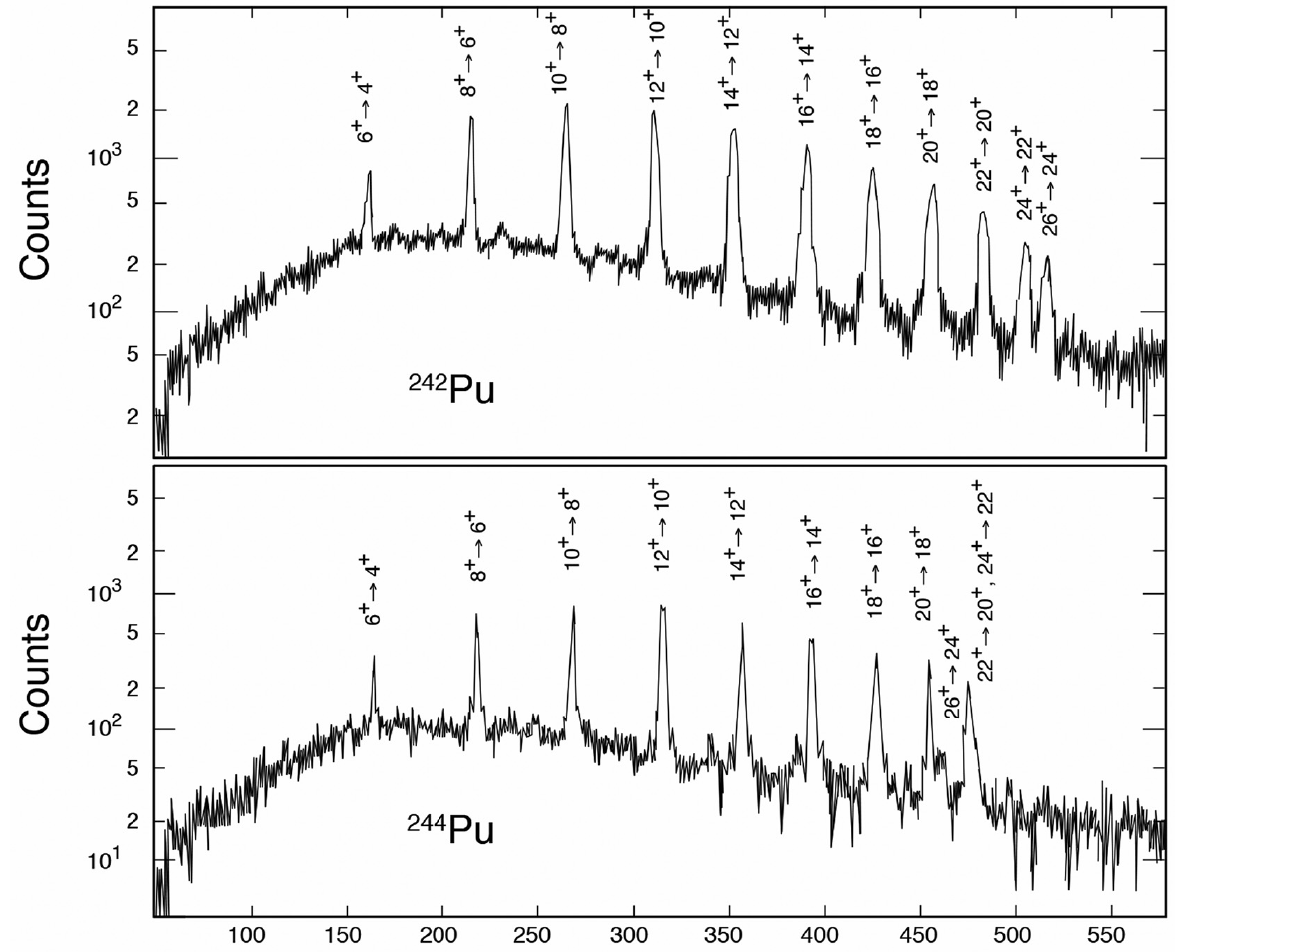
\includegraphics[width=\linewidth]{assets/2.1.3_Pu_shifts.png}
    \end{minipage}
    \hfill
    \begin{minipage}[b]{0.48\textwidth}
        \centering
        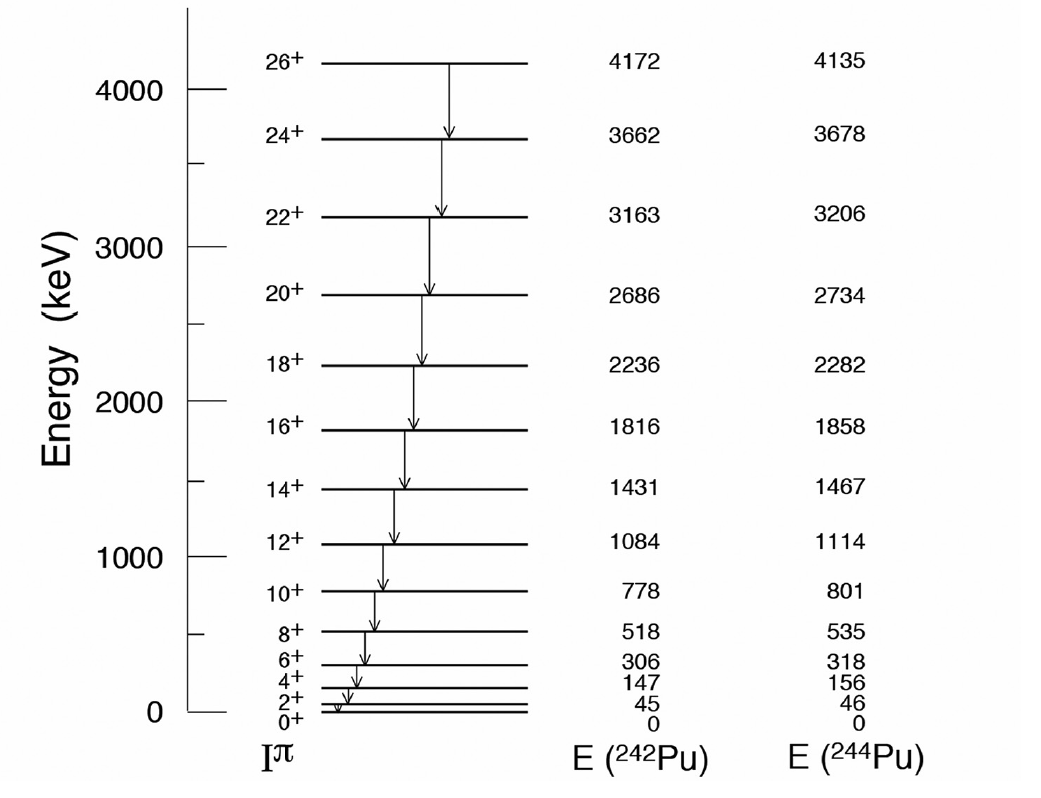
\includegraphics[width=\linewidth]{assets/2.1.3_Pu_levels.png}
    \end{minipage}



\allbold{Scale the excitation energies to that of \(2_1^+\) states i.e. divide the energies for \ce{^{242}Pu} by \(45\) and \ce{^{244}Pu} by \(46\). Having scaled the energies, plot the two bands as \(E(I_{\text{scaled}})\) vs \(I(I+1)\). Note that, while the energies look significantly different, when scaled they are nearly identical i.e. there is evidently some underlying universal rotational energy profile. This does not appear to have been recognised, but holds for the most strongly deformed ground-sate bands, extending into the rare earth region e.g. \ce{^{174}Yb}. Higher precision energy values can be used but this exercise captures the essence of the feature.}

\begin{center}
\begin{tabular}{rrrrrr}
\toprule
$I$ & $I(I+1)$ & E(\ce{^{242}Pu}) & E\(_{\text{scaled}}\)(\ce{^{242}Pu}) & E(\ce{^{244}Pu}) & E\(_{\text{scaled}}\)(\ce{^{242}Pu}) \\
\midrule
2  & 6   & 45   & 1.00  & 46   & 1.00  \\
4  & 20  & 147  & 3.27  & 156  & 3.39  \\
6  & 42  & 306  & 6.80  & 318  & 6.91  \\
8  & 72  & 518  & 11.51 & 535  & 11.63 \\
10 & 110 & 778  & 17.29 & 801  & 17.41 \\
12 & 156 & 1084 & 24.09 & 1114 & 24.22 \\
14 & 210 & 1431 & 31.80 & 1467 & 31.89 \\
16 & 272 & 1816 & 40.36 & 1858 & 40.39 \\
18 & 342 & 2236 & 49.69 & 2282 & 49.61 \\
20 & 420 & 2686 & 59.69 & 2734 & 59.43 \\
22 & 506 & 3163 & 70.29 & 3206 & 69.70 \\
24 & 600 & 3662 & 81.38 & 3678 & 79.96 \\
26 & 702 & 4172 & 92.71 & 4135 & 89.89 \\
\bottomrule
\end{tabular}
\end{center}

\begin{tikzpicture}
\begin{axis}[
    width=0.85\textwidth,
    height=0.6\textwidth,
    xlabel={$I(I+1)$},
    ylabel={Energy Scaled to E(\(2_1^+\)) / keV},
    xmin=0, xmax=750,
    ymin=0, ymax=100,
    grid=major,
    grid style={dotted,gray!50},
    legend pos=north west,
    legend cell align={left},
    mark size=2pt,
]

% Rigid rotor guide: E_scaled = I(I+1)/6
\addplot[black, dashed, no markers, domain=0:750] {x/6};
\addlegendentry{$I(I+1)/6$ (rigid rotor)}

% 242Pu
\addplot[blue, mark=*, thick] coordinates {
    (6,1.00) (20,3.27) (42,6.80) (72,11.51) (110,17.29)
    (156,24.09) (210,31.80) (272,40.36) (342,49.69)
    (420,59.69) (506,70.29) (600,81.38) (702,92.71)
};
\addlegendentry{\ce{^{242}Pu}}

% 244Pu
\addplot[red, mark=square*, thick] coordinates {
    (6,1.00) (20,3.39) (42,6.91) (72,11.63) (110,17.41)
    (156,24.22) (210,31.89) (272,40.39) (342,49.61)
    (420,59.43) (506,69.70) (600,79.96) (702,89.89)
};
\addlegendentry{\ce{^{244}Pu}}

\end{axis}
\end{tikzpicture}
\end{example}

\begin{example}{3}{3-6: Exploring the Nuclear Structure of \ce{^{175}Lu} with ENSDF Pages}
    
\end{example}